\documentclass[a4paper,12pt]{article}
\usepackage[utf8]{inputenc}
\usepackage{graphicx}
\usepackage{fancyhdr}
\usepackage{amsmath}
\usepackage{adjustbox}
\usepackage{mathtools}
\usepackage{float}
\usepackage[spanish]{babel} 
\usepackage{lastpage}
\usepackage{amssymb} % Para símbolos matemáticos adicionales
\usepackage{cleveref}
%\usepackage[none]{hyphenat}
\usepackage{array}

\usepackage{multirow}
\usepackage{textcomp}
\usepackage[left=2.5cm, right=2.5cm, top=3cm, bottom=3cm]{geometry}

\graphicspath{{Imagenes/}}

% Encabezado y pie de página
\pagestyle{fancy}
\fancyhf{}
\setlength{\headheight}{30 pt}
\renewcommand{\headrulewidth}{0.2pt}
\fancyhead[R]{\begin{tabular}{@{}l@{}}
\includegraphics[scale=0.4]{escudo.PNG}\end{tabular}}
\fancyhead[L]{\begin{tabular}{@{}c@{}} \textbf{Robótica I - Año: 2024} \\ Trabajo Práctico 3: Denavit y Hartenberg \end{tabular}}


\fancyfoot[R]{\thepage}
\fancyfoot[C]{\begin{tabular}{@{}c@{}}\textbf{BORQUEZ PEREZ Juan Manuel}\\ \textbf{Legajo 13567}\end{tabular}}
\renewcommand{\footrulewidth}{0.2pt}

\begin{document}

\begin{titlepage}
    \centering
    \vspace*{5cm}
    {\Huge\bfseries Informe de Trabajo Práctico N°3}\\
    \vspace{0.2cm}
    {\Large \textbf{Denavit y Hartenberg}}\\
    \vspace{0.5cm}
    {\Large Robótica I}\\
    \vspace{0.5 cm}
    {\Large Ingeniería en Mecatrónica}\\
    \vspace{0.2 cm}
    {\Large Facultad de Ingeniería - UNCUYO}\\
    \vspace{1.5cm}
    Alumno: Juan Manuel BORQUEZ PEREZ\\
    Legajo: 13567\\
    \vfill
    {\begin{tabular}{@{}c@{}}
\includegraphics[scale=0.4]{escudo.PNG}\end{tabular}}\hspace{10pt}
    %Año 2023
\end{titlepage}

\section{Ejercicio 1.}
La convención de Denavit - Hartenberg (DH) se utiliza para establecer una matriz
de transformación homogénea que describe la posición y orientación de un sistema de
referencia respecto a otro, y está formada por el producto de 4 transformaciones elementales,
2 traslaciones y 2 rotaciones. Considere que existen algunas modificaciones de la convención
original, pero en este cursado usaremos la estándar (prestar atención a las indicaciones de los
autores al momento de presentarla).

\subsection{Inciso 1.}
\textbf{Escriba de forma simbólica cada transformación elemental, indicando si es
traslación o rotación, el parámetro principal, y con respecto a qué eje se realiza}

\begin{enumerate}
    \item Rotación alrededor del eje $Z_{i-1}$ un ángulo $\theta_i$ para llevar el eje $X_{i-1}$ hasta el eje $X_i$. Corresponde con la variable articular $q_i$.
    \[Rot\left(Z_{i-1}, \theta_i\right)\]
    \item Traslación a lo largo de $Z_{i-1}$ una distancia $d_i$ desde el origen del sistema $\{S_{i-1}\}$ hasta el eje $X_i$. Corresponde con la longitud articular.
    \[Tras\left(Z_{i-1}, d_i\right)\]
    \item Traslación a lo largo del eje $X_i$ una distancia $a_i$ desde el eje $Z_{i-1}$ al eje $Z_{i}$. Corresponde con la longitud del eslabón $i$.
    \[Tras\left(X_{i}, a_i\right)\]
    \item Rotación alrededor del eje $X_{i}$ un ángulo $\alpha_i$ desde el eje $Z_{i-1}$ al eje $Z_{i}$. Corresponde con el ángulo de torsión del eslabon $i$.
    \[Rot\left(X_{i}, \alpha_i\right)\]
\end{enumerate}

\subsection{Inciso 2.}
\textbf{Escriba el producto matricial ordenado y la forma general de la matriz homogénea
que relaciona 2 sistemas consecutivos}

\[\prescript{i-1}{}{T_i} = Rot\left(Z_{i-1}, \theta_i\right) Tras\left(Z_{i-1}, d_i\right) Tras\left(X_{i}, a_i\right) Rot\left(X_{i}, \alpha_i\right)\]

\section{Ejercicio 2}
\textbf{Aplique la convención DH a los siguientes robots. Es decir, asigne adecuadamente
los sistemas de referencia y determine los 4 parámetros de cada articulación: $\theta$, $d$, $a$, $\alpha$. Realice
un esquema adecuado donde se aprecien todos los parámetros involucrados.}

\subsection{Inciso 1}

\begin{figure}[H]
    \centering
    \begin{adjustbox}{scale = 0.5, max width=\columnwidth}
        \framebox{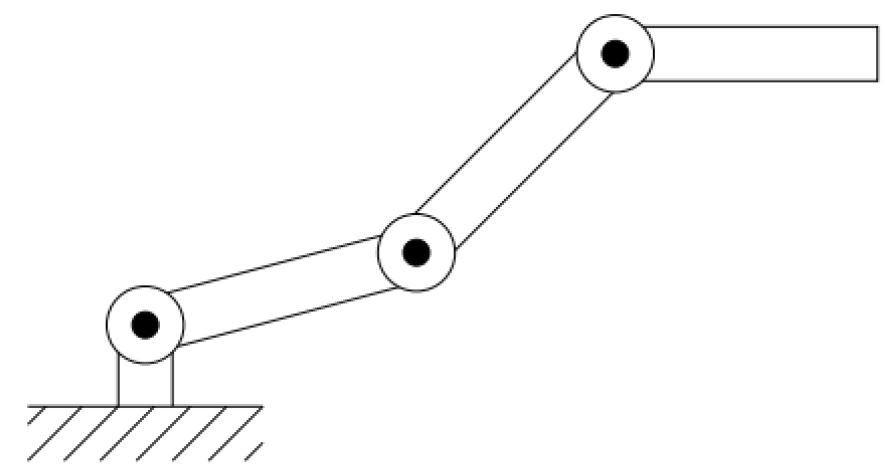
\includegraphics{1-Ejercicio_2_1_enunciado.JPG}}
    \end{adjustbox}
    \caption{Robot planar de 3 articulaciones rotacionales (Spong 2005).}
\end{figure}

\begin{figure}[H]
    \centering
    \begin{adjustbox}{scale = 0.5, max width=\columnwidth}
        \framebox{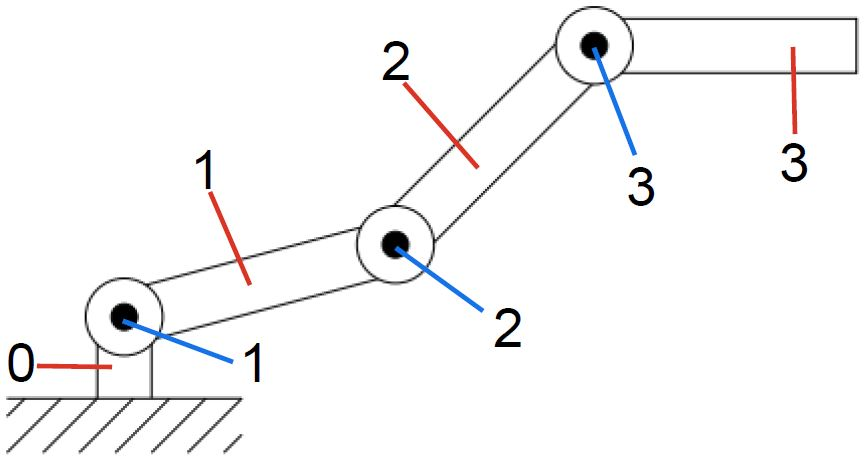
\includegraphics{2-Ejercicio_2_1_eslabones_articulaciones.JPG}}
    \end{adjustbox}
    \caption{Identificación de eslabones y articulaciones.}
\end{figure}

\begin{figure}[H]
    \centering
    \begin{adjustbox}{scale = 0.6, max width=\columnwidth}
        \framebox{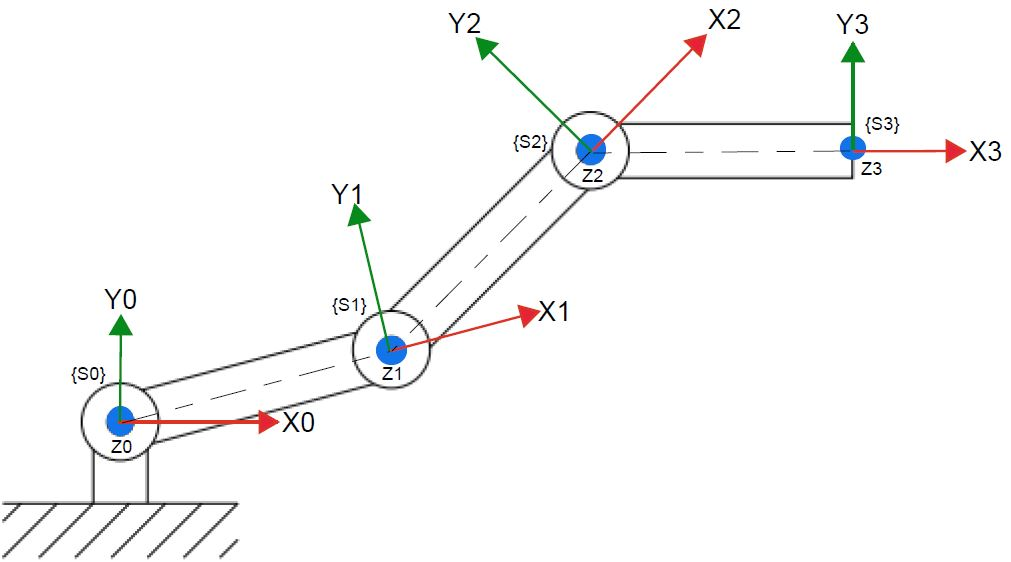
\includegraphics{3-Ejercicio_2_1_sistemas.JPG}}
    \end{adjustbox}
    \caption{Definición de los sistemas.}
\end{figure}

\begin{figure}[H]
    \centering
    \begin{adjustbox}{scale = 0.58, max width=\columnwidth}
        \framebox{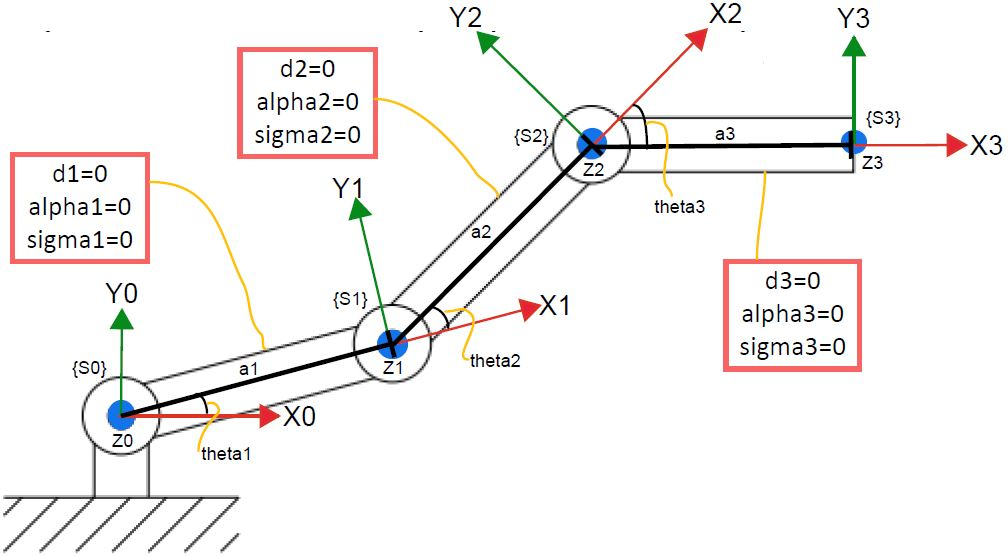
\includegraphics{4-Ejercicio_2_1_DH.JPG}}
    \end{adjustbox}
    \caption{Aplicación de la convención DH.}
\end{figure}

\begin{table}[H]
    \centering
    \begin{tabular}{|c|c|c|c|c|c|}
    \hline
    Sistema & $\theta$ & $d$ & $a$         & $\alpha$ & $\sigma$ \\ \hline
    1       & $q_1$     & 0   & $l_{esl1}$  & 0        & 0        \\ \hline
    2       & $q_2$     & 0   & $l_{esl2}$  & 0        & 0        \\ \hline
    3       & $q_3$     & 0   & $l_{esl3}$  & 0        & 0        \\ \hline
    \end{tabular}
    \caption{Síntesis de la convención DH.}
\end{table}

\subsection{Inciso 2.}

\begin{figure}[H]
    \centering
    \begin{adjustbox}{scale = 0.5, max width=\columnwidth}
        \framebox{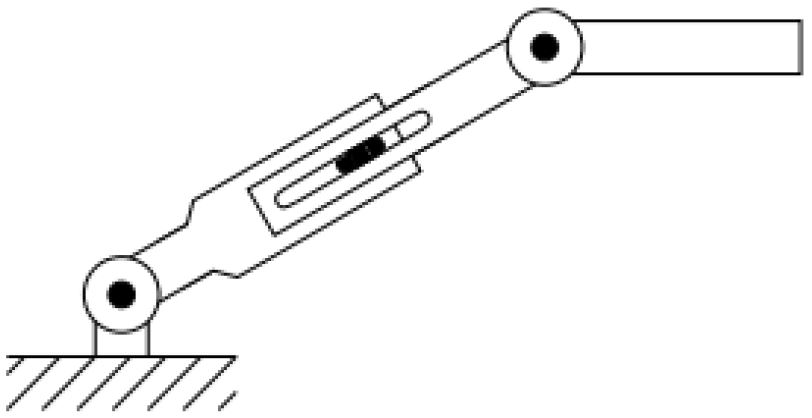
\includegraphics{5-Ejercicio_2_2_enunciado.JPG}}
    \end{adjustbox}
    \caption{Robot planar con 3 articulaciones: rotación, traslación, rotación (Spong 2005).}
\end{figure}

\begin{figure}[H]
    \centering
    \begin{adjustbox}{scale = 0.5, max width=\columnwidth}
        \framebox{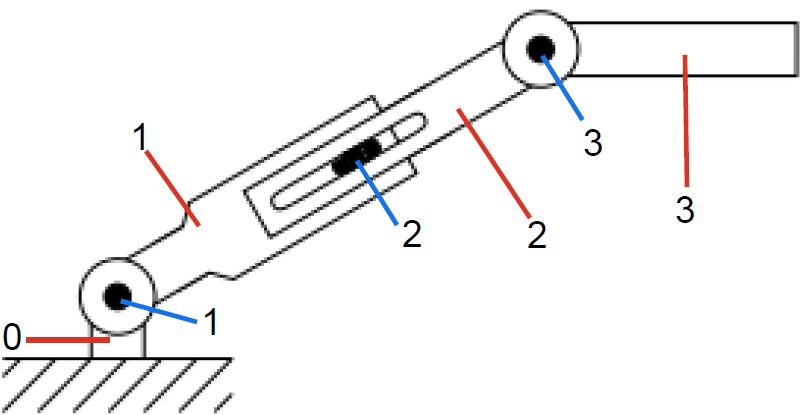
\includegraphics{6-Ejercicio_2_2_eslabones_articulaciones.JPG}}
    \end{adjustbox}
    \caption{Identificación de eslabones y articulaciones.}
\end{figure}

\begin{figure}[H]
    \centering
    \begin{adjustbox}{scale = 0.5, max width=\columnwidth}
        \framebox{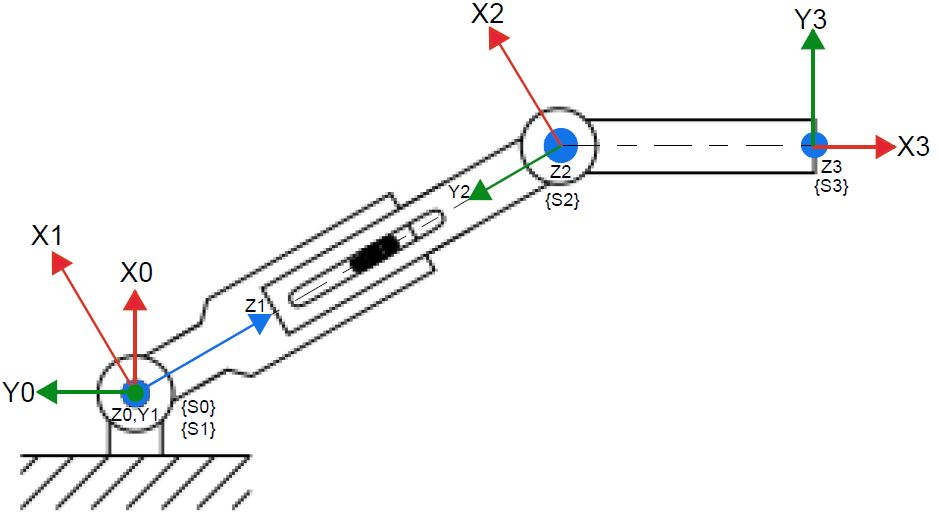
\includegraphics{7-Ejercicio_2_2_sistemas.JPG}}
    \end{adjustbox}
    \caption{Definición de los sistemas.}
\end{figure}

\begin{figure}[H]
    \centering
    \begin{adjustbox}{scale = 0.85, max width=\columnwidth}
        \framebox{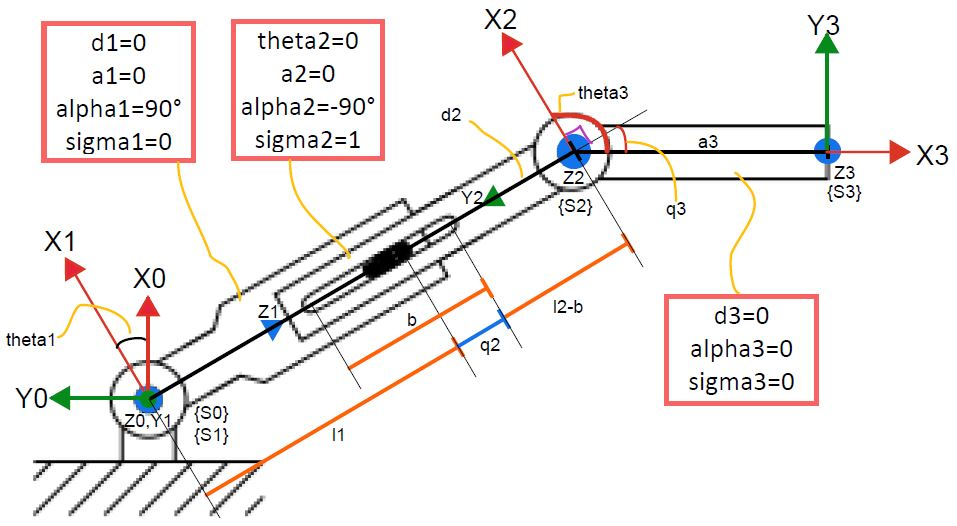
\includegraphics{8-Ejercicio_2_2_DH.JPG}}
    \end{adjustbox}
    \caption{Aplicación de la convención DH.}
\end{figure}

\begin{table}[H]
    \centering
    \begin{tabular}{|c|c|c|c|c|c|}
    \hline
    Sistema & $\theta$          & $d$                               & $a$         & $\alpha$     & $\sigma$ \\ \hline
    1       & $q_1$             & 0                                 & $0$         & $90^\circ$   & 0        \\ \hline
    2       & $0$               & $q_2 + l_{esl1} + l_{esl2} - b$   & $0$         & $-90^\circ$  & 1        \\ \hline
    3       & $q_3 - 90^\circ$  & 0                                 & $l_{esl3}$  & 0            & 0        \\ \hline
    \end{tabular}
    \caption{Síntesis de la convención DH.}
\end{table}

\subsection{Inciso 3.}

\begin{figure}[H]
    \centering
    \begin{adjustbox}{scale = 0.7, max width=\columnwidth}
        \framebox{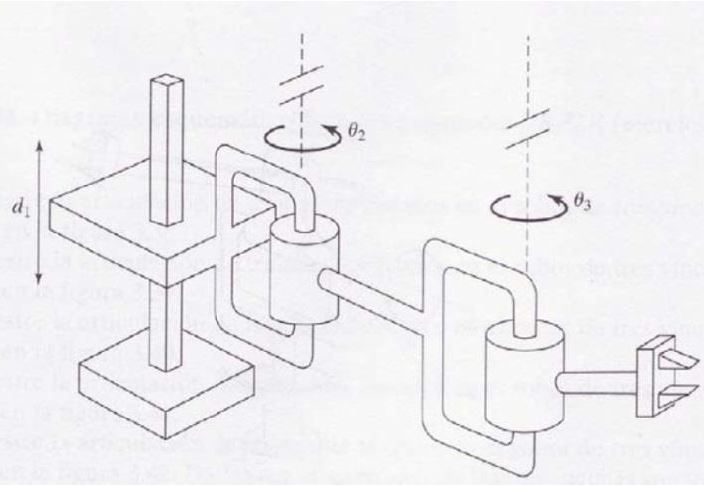
\includegraphics{9-Ejercicio_2_3_enunciado.JPG}}
    \end{adjustbox}
    \caption{Robot de 3 articulaciones: traslación, rotación, rotación (Craig 2006)}
\end{figure}

\begin{figure}[H]
    \centering
    \begin{adjustbox}{scale = 0.7, max width=\columnwidth}
        \framebox{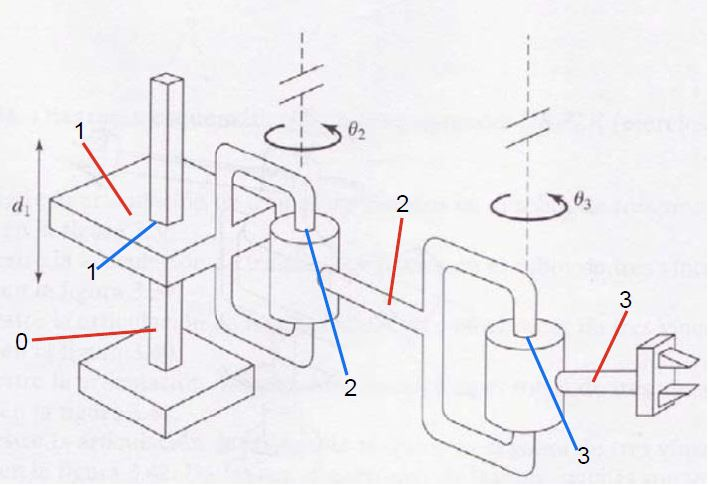
\includegraphics{10-Ejercicio_2_3_eslabones_articulaciones.JPG}}
    \end{adjustbox}
    \caption{Identificación de eslabones y articulaciones.}
\end{figure}

\begin{figure}[H]
    \centering
    \begin{adjustbox}{scale = 0.66, max width=\columnwidth}
        \framebox{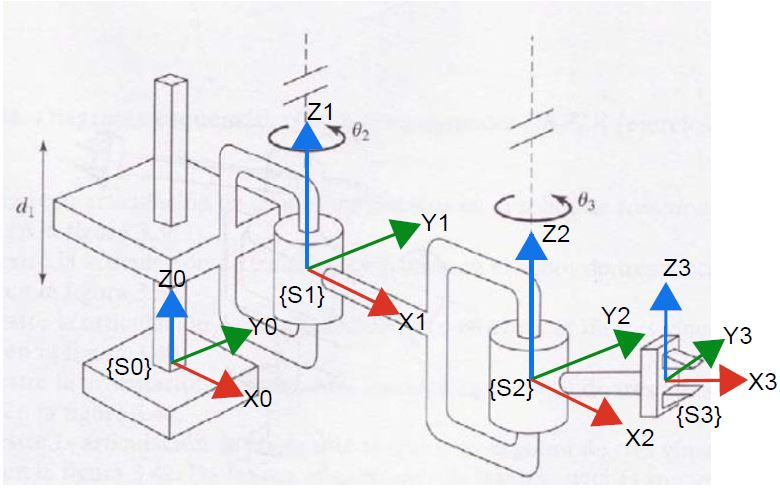
\includegraphics{11-Ejercicio_2_3_sistemas.JPG}}
    \end{adjustbox}
    \caption{Definición de los sistemas.}
\end{figure}

\begin{figure}[H]
    \centering
    \begin{adjustbox}{scale = 0.66, max width=\columnwidth}
        \framebox{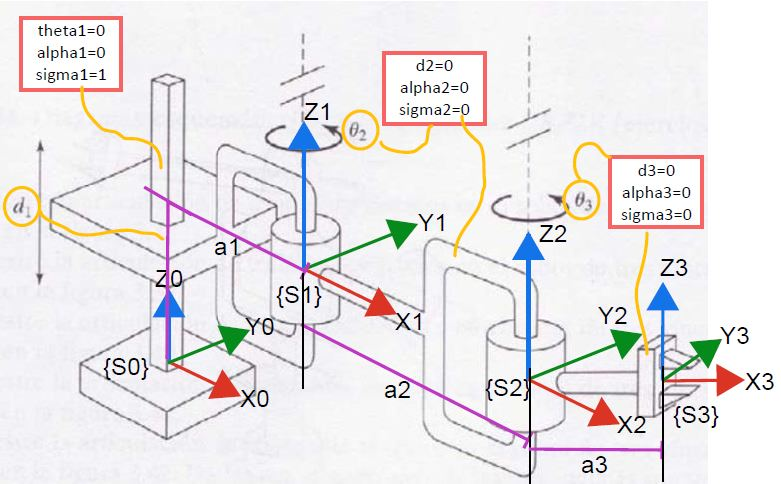
\includegraphics{12-Ejercicio_2_3_DH.JPG}}
    \end{adjustbox}
    \caption{Aplicación de la convención DH.}
\end{figure}

\begin{table}[H]
    \centering
    \begin{tabular}{|c|c|c|c|c|c|}
    \hline
    Sistema & $\theta$  & $d$ & $a$         & $\alpha$ & $\sigma$ \\ \hline
    1       & $0$       & $d_1$ & $l_{esl1}$  & 0      & 1        \\ \hline
    2       & $q_2$     & 0   & $l_{esl2}$  & 0        & 0        \\ \hline
    3       & $q_3$     & 0   & $l_{esl3}$  & 0        & 0        \\ \hline
    \end{tabular}
    \caption{Síntesis de la convención DH.}
\end{table}

\section{Ejercicio 3.}
\textbf{Determine los parámetros DH de cada uno de los siguientes robots reales. Analice
cada uno de ellos y obtenga los datos necesarios de su geometría a partir de la información
gratuita que el fabricante pone a disposición en su página web. Si existe más de un modelo
para cada caso seleccione uno, cualquiera.}

\subsection{SCARA IRB 910SC-3/0.45 (ABB).}

\begin{figure}[H]
    \centering
    \begin{adjustbox}{scale = 0.662, max width=\columnwidth}
        \framebox{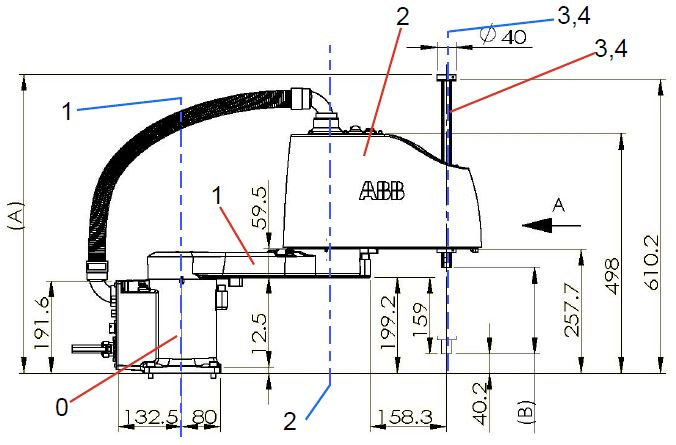
\includegraphics{13-Ejercicio_3_1_eslabones_articulaciones.JPG}}
    \end{adjustbox}
    \caption{Identificación de eslabones y articulaciones.}
    \label{scara_eslabones_articulaciones}
\end{figure}

\begin{figure}[H]
    \centering
    \begin{adjustbox}{scale = 0.662, max width=\columnwidth}
        \framebox{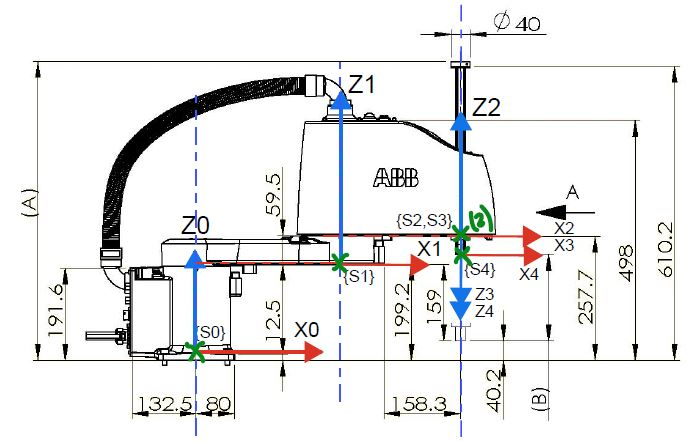
\includegraphics{14-Ejercicio_3_1_sistemas_lateral.JPG}}
    \end{adjustbox}
    \caption{Definición de sistemas vista lateral.}
    \label{scara_sistemas_lateral}
\end{figure}

Como se puede ver en las \cref{scara_eslabones_articulaciones}, \cref{scara_sistemas_lateral} y \cref{scara_sistemas_superior},
hemos separado al par cilíndrico en el extremo del robot por un par de rotación más un par prismático
y hemos considerado un sistema de referencia independiente para cada uno (\{S2\} y \{S3\}).

\begin{figure}[H]
    \centering
    \begin{adjustbox}{scale = 0.7, max width=\columnwidth}
        \framebox{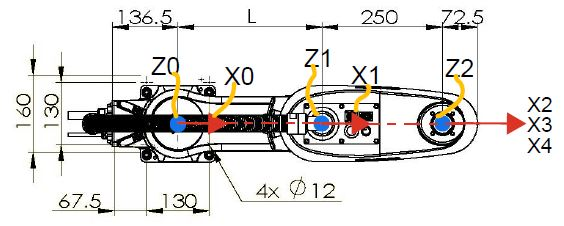
\includegraphics{15-Ejercicio_3_1_sistemas_superior.JPG}}
    \end{adjustbox}
    \caption{Definición de los sistemas vista superior.}
    \label{scara_sistemas_superior}
\end{figure}

Los parámetros para la convención DH se resaltaron en las \cref{DH_superior} y \cref{DH_lateral}
con cuadros de color violeta para las dimensiones en milímetros y con cuadros en rojo
para la denominación de los parámetros; mientras que aquellos parámetros que no se indican en las figuras
se colocan directamente en la \cref{sintesis_DH_scara}. En la \cref{DH_lateral} también se indica en forma
de árbol la cuenta que hay que hacer para determinar $d_4$.

\begin{figure}[H]
    \centering
    \begin{adjustbox}{scale = 0.66, max width=\columnwidth}
        \framebox{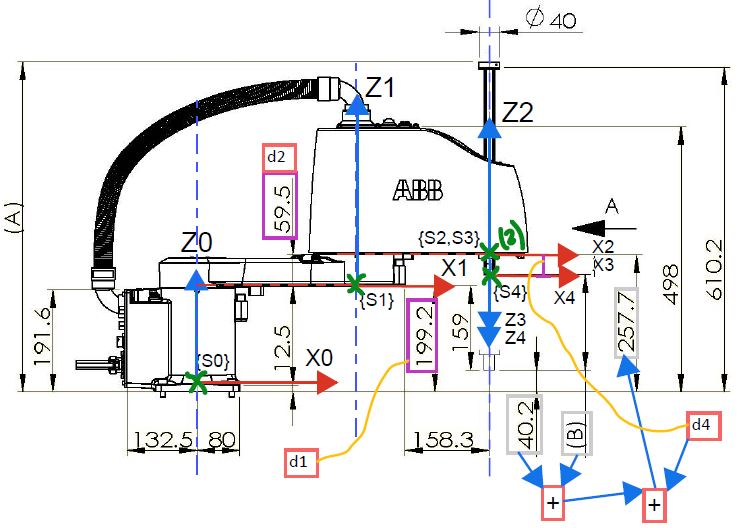
\includegraphics{16-Ejercicio_3_1_DH_lateral.JPG}}
    \end{adjustbox}
    \caption{Aplicación de la convención DH vista lateral.}
    \label{DH_lateral}
\end{figure}

\begin{figure}[H]
    \centering
    \begin{adjustbox}{scale = 0.66, max width=\columnwidth}
        \framebox{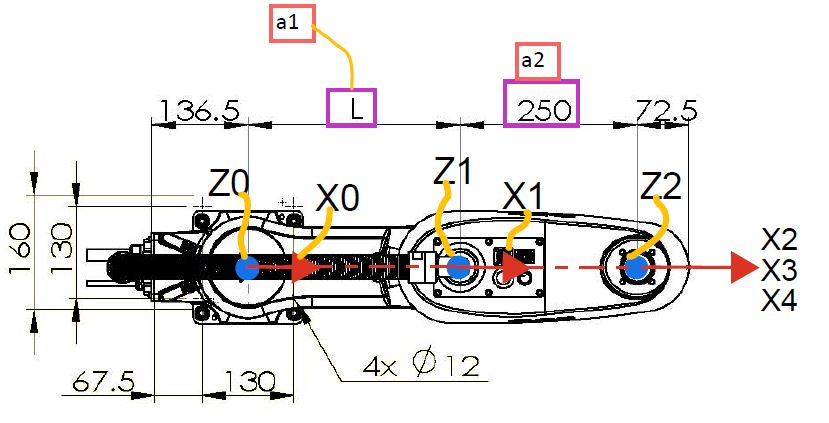
\includegraphics{17-Ejercicio_3_1_DH_superior.JPG}}
    \end{adjustbox}
    \caption{Aplicación de la convención DH vista superior.}
    \label{DH_superior}
\end{figure}

\begin{figure}[H]
    \centering
    \begin{adjustbox}{scale = 0.66, max width=\columnwidth}
        \framebox{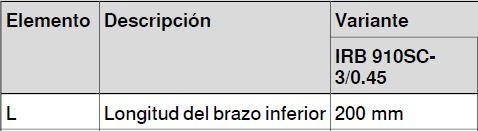
\includegraphics{18-Ejercicio_3_1_DH_parametros_dsh.JPG}}
    \end{adjustbox}
    \caption{parámetros 1.}
\end{figure}

\begin{figure}[H]
    \centering
    \begin{adjustbox}{scale = 0.66, max width=\columnwidth}
        \framebox{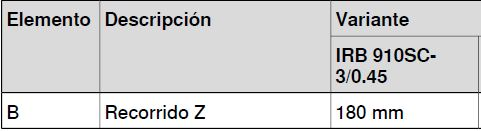
\includegraphics{19-Ejercicio_3_1_DH_parametros_dsh.JPG}}
    \end{adjustbox}
    \caption{parámetros 2.}
\end{figure}

\begin{table}[H]
    \centering
    \begin{tabular}{|c|c|c|c|c|c|}
    \hline
    Sistema & $\theta$  & $d$           & $a$    & $\alpha$ & $\sigma$ \\ \hline
    1       & $q_1$     & $199.2$       & $200$  & 0        & 0        \\ \hline
    2       & $q_2$     & $59.5$        & $250$  & 0        & 0        \\ \hline
    3       & $q_3$     & $0$           & $0$    & 90°      & 0        \\ \hline
    4       & $0$       & $37.5 + q_4$  & $0$    & 0        & 1        \\ \hline
    \end{tabular}
    \caption{Síntesis de la convención DH.}
    \label{sintesis_DH_scara}
\end{table}

\subsection{Paint Mate 200iA (FANUC).}

\subsection{LBR iiwa 7 R800 (KUKA).}

\end{document}

%\begin{equation*}
%    \prescript{O}{}{Rot_M} = 
%    \begin{bmatrix}
%        0.500 & -0.866\\
%        0.866 & 0.500
%    \end{bmatrix}
%\end{equation*}

%\begin{figure}[H]
%    \centering
%    \begin{adjustbox}{scale = 0.85, max width=\columnwidth}
%        \framebox{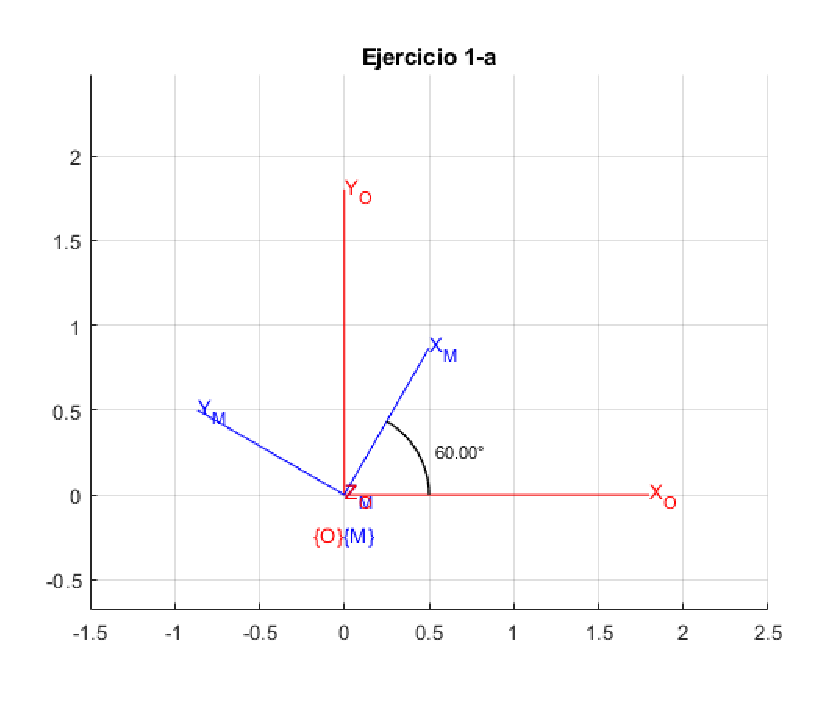
\includegraphics{1-Ejercicio_1_a.pdf}}
%    \end{adjustbox}
%    \caption{Sistema O y Sistema M superpuestos con indicación de ángulo de rotación.}
%\end{figure}

\end{document}